% ============================================================
% RESULTS (part A): corpus, rules vs learned, feature views
% ============================================================
\section{Results and Discussion}

\subsection{Corpus Statistics}

Building the corpus is cheap. Generating the \NProg{} programs, including the compilation that checks each fault
for manifestation, took 18 seconds, and extracting the feature vectors another 3 seconds on ten worker processes. The
operator table in Appendix~C shows that most operators are applicable to most programs; the lowest yields come from
operators that need a particular construct to be present (for example \code{unit\_return} needs the BMI function,
\code{phi\_removeanon} needs an existing \code{anonymize} call). Among the faulty programs, \DoubleShare\% contain two
faults.

\subsection{Rule-Based Diagnostics versus Learned Classification (E1)}

Table~\ref{tab:rulesml} compares the two rule baselines with the four learned classifiers on the \NTest{} test programs.
The learned models reach between \RFAcc\% (random forest) and \HGBAcc\% (gradient boosting) accuracy, against
\RuleFirstAcc\% for the ``first error'' rule and \RulePrioAcc\% for the ``most severe family'' rule. The four learned
models are within 0.3 percentage points of each other, which on 2{,}000 test programs is a difference of six programs; we
do not read any ranking into it. We use the random forest in the remainder of the report because it is the model deployed
in the command-line tool and because its feature importances are easy to inspect.

\begin{table}[H]
\centering
\caption{Test-set performance of the rule baselines and the learned classifiers
(\NTest{} test programs; trained on \NTrain{} programs).}
\label{tab:rulesml}
\small
\begin{tabular}{lrrrr}
\toprule
\textbf{Classifier} & \textbf{Accuracy} & \textbf{Macro-F1} & \textbf{Acc.\ single-fault} & \textbf{Acc.\ two-fault}\\
\midrule
Rule: first error & 0.9160 & 0.9157 & 0.9623 & 0.6568\\
Rule: most severe family & 0.9320 & 0.9299 & 0.9275 & 0.9571\\
Random forest & 0.9915 & 0.9915 & 0.9965 & 0.9637\\
MLP & 0.9935 & 0.9935 & 0.9976 & 0.9703\\
LogReg & 0.9920 & 0.9920 & 0.9971 & 0.9637\\
HistGB & 0.9940 & 0.9940 & 0.9959 & 0.9835\\\bottomrule
\end{tabular}

\end{table}

The error breakdown in Figure~\ref{fig:confusion} and Table~\ref{tab:perclass} shows \emph{where} the rules fall short.

\begin{figure}[H]
\centering
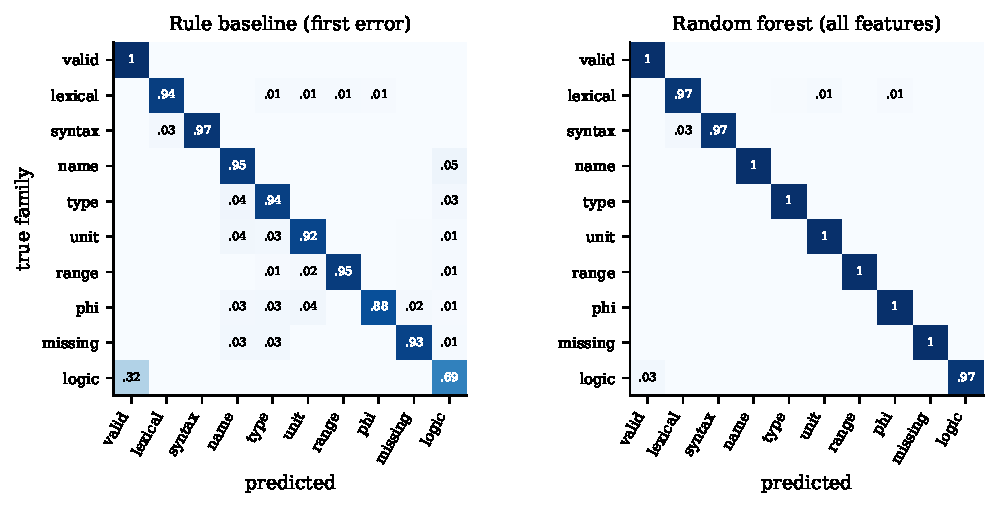
\includegraphics[width=\textwidth]{figs/confusion.pdf}
\caption{Row-normalised confusion matrices on the test set. Left: the ``first error'' rule. Right: random forest.}
\label{fig:confusion}
\end{figure}

\begin{table}[H]
\centering
\caption{Per-class F1 of the rule baselines and precision, recall and F1 of the random forest.}
\label{tab:perclass}
\small
\begin{tabular}{lrrrrr}
\toprule
 & \multicolumn{2}{c}{\textbf{Rule F1}} & \multicolumn{3}{c}{\textbf{Random forest}}\\
\cmidrule(lr){2-3}\cmidrule(lr){4-6}
\textbf{Family} & first & severe & P & R & F1\\
\midrule
valid & 0.864 & 0.864 & 0.971 & 1.000 & 0.985\\
lexical & 0.959 & 0.777 & 0.975 & 0.970 & 0.972\\
syntax & 0.987 & 0.846 & 1.000 & 0.975 & 0.987\\
name & 0.913 & 1.000 & 1.000 & 1.000 & 1.000\\
type & 0.912 & 1.000 & 0.995 & 1.000 & 0.998\\
unit & 0.922 & 1.000 & 0.985 & 1.000 & 0.993\\
range & 0.967 & 1.000 & 1.000 & 1.000 & 1.000\\
phi & 0.931 & 1.000 & 0.990 & 1.000 & 0.995\\
missing & 0.946 & 1.000 & 1.000 & 1.000 & 1.000\\
logic & 0.755 & 0.813 & 1.000 & 0.970 & 0.985\\\bottomrule
\end{tabular}

\end{table}

\begin{enumerate}
    \item \textbf{Faults the compiler cannot see.} 63 of the 200 test programs in the \emph{logic} class (31.5\%) are
    reported as clean by both rules, so their \emph{logic} recall is only \RuleLogicRecall\%. These are the inverted
    clinical rules and the mismatched alert texts: the programs are well formed, well typed and unit-correct. The random
    forest recovers them (\RFLogicRecall\% recall for \emph{logic}) using the pattern features, which count relational
    operators that point the wrong way relative to the alert vocabulary nearby. Six \emph{logic} programs are still
    taken for \emph{valid}.
    \item \textbf{Cascades hide the root cause of lexical faults.} The ``most severe family'' rule is perfect on all six
    semantic families, which is unsurprising because it implements the labelling rule. It fails on \emph{lexical}
    programs: an unterminated string swallows the rest of its line, the parser then reports follow-on syntax errors, and
    the priority rule, which ranks syntax above lexical, picks the symptom (73 of 200 programs). The ``first error''
    rule gets these right more often because the lexical error is reported first, but it pays for that elsewhere.
    \item \textbf{The first diagnostic is not always the root cause.} With two faults in the program, the ``first error''
    rule is correct on only \RuleFirstDouble\% of them, against 96.2\% on single-fault programs; the random forest is correct on
    \RFDouble\% of the two-fault programs.
    \item \textbf{What remains.} The forest makes 17 errors on 2{,}000 programs: six \emph{logic} programs taken for
    \emph{valid} (the soft faults above), five \emph{syntax} programs taken for \emph{lexical}, and six \emph{lexical}
    programs assigned to a semantic family (one \emph{type}, three \emph{unit}, two \emph{phi}). The lexical--syntax
    confusion is the same cascade ambiguity as before and is not fully resolved.
\end{enumerate}

None of this says that machine learning is better than a well-designed rule set \emph{for the faults the rules were
written for}: on those, a precise analyser is already at 100\%. The gain is concentrated in the cases that a
rule-based analyser misses or mislabels. It is also worth being clear about what the 99\% figure means. The test programs
come from the same generator as the training programs, so the learned model is evaluated on an in-distribution
sample; Section~5.8 discusses what that does and does not show.

\paragraph{What the forest relies on.} Table~\ref{tab:topfeat} lists the most important features. The most important one by a
wide margin is \code{worst\_family\_rank}, the compiler-derived rank of the most severe diagnostic family; the next ones are
counts of individual diagnostic codes. In other words, the learned classifier is largely a learned post-processor of the
compiler's output---which is what the architecture intends.

\begin{table}[H]
\centering
\caption{Top-eight random-forest feature importances (mean decrease in impurity).}
\label{tab:topfeat}
\small
\begin{tabular}{lr}
\toprule
\textbf{Feature} & \textbf{Importance}\\
\midrule
\texttt{worst\_family\_rank} & 0.142\\
\texttt{diag\_DOM002} & 0.053\\
\texttt{diag\_DOM001} & 0.051\\
\texttt{first\_phase\_sem} & 0.048\\
\texttt{diag\_SEM005} & 0.044\\
\texttt{first\_fam\_type} & 0.043\\
\texttt{diag\_DOM003} & 0.043\\
\texttt{first\_fam\_name} & 0.039\\\bottomrule
\end{tabular}

\end{table}

\subsection{Which Feature Groups Matter, and How Much Data Is Needed (E2)}

Figure~\ref{fig:learning} and Table~\ref{tab:learning} show test macro-F1 of a random forest trained on four feature
views with an increasing number of training programs per class (mean over five random draws).

\begin{figure}[H]
\centering
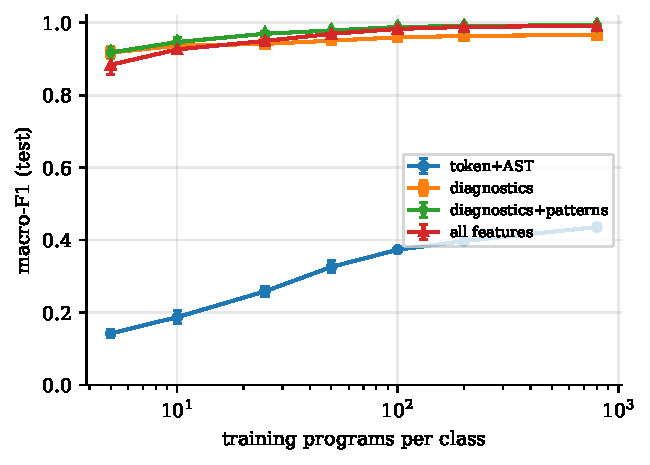
\includegraphics[width=0.62\textwidth]{figs/learning.pdf}
\caption{Learning curves of the random forest for four feature views (mean $\pm$ standard deviation over five draws).}
\label{fig:learning}
\end{figure}

\begin{table}[H]
\centering
\caption{Test macro-F1 by feature view and number of training programs per class.}
\label{tab:learning}
\small
\resizebox{\textwidth}{!}{\begin{tabular}{lrrrrrrr}
\toprule
\textbf{Feature view} & \textbf{5} & \textbf{10} & \textbf{25} & \textbf{50} & \textbf{100} & \textbf{200} & \textbf{800}\\
\midrule
token+AST & 0.142 & 0.187 & 0.258 & 0.326 & 0.373 & 0.398 & 0.436\\
diagnostics & 0.918 & 0.937 & 0.942 & 0.950 & 0.960 & 0.963 & 0.967\\
diagnostics+patterns & 0.918 & 0.946 & 0.970 & 0.979 & 0.988 & 0.991 & 0.994\\
all features & 0.884 & 0.926 & 0.950 & 0.969 & 0.983 & 0.988 & 0.991\\\bottomrule
\end{tabular}
}
\end{table}

Three observations follow.

\begin{itemize}
    \item \textbf{Surface features are not enough.} Token and tree statistics alone give a macro-F1 of only 0.14 with five
    programs per class and 0.44 with 800. A forest cannot recover from raw counts what a unit checker or a taint analysis
    computes. This is the strongest argument in the data for putting a real compiler front end underneath the learner.
    \item \textbf{Diagnostics carry most of the signal; patterns add the rest.} The diagnostic features alone plateau at
    0.967: they cannot see the soft logic faults. Adding the six pattern features lifts the curve to 0.994 at 800 programs per
    class.
    \item \textbf{More features are not better at small sample sizes.} The ``all features'' view is slightly \emph{worse}
    than diagnostics$+$patterns at every size (0.884 versus 0.918 at five programs per class, 0.991 versus 0.994 at 800). The
    token and tree features add 55 noisy dimensions that carry little information. We nevertheless kept the full 101-dimensional
    vector for the experiments with the GAN, because it is the representation the deployed classifier uses; a leaner view would be
    a reasonable simplification.
\end{itemize}

The scarce-data end of the curve is where it matters for the next experiment: with five labelled programs per class a forest
reaches a macro-F1 of 0.88, and the question is whether synthetic records can close part of the gap to 0.99.

